\section{666 --- Path Sum IV}
If the depth of a tree is smaller than \textcolor{red}{5}, then this tree can be represented by a list of three-digits integers.

For each integer in this list:

\begin{enumerate}
\item The hundreds digit represents the depth $D$ of this node, $1 \leq D \leq 4$.
\item The tens digit represents the position $P$ of this node in the level it belongs to, $1 \leq P \leq 8$. The position is the same as that in a full binary tree.
\item The units digit represents the value $V$ of this node, $0 \leq V \leq 9$.

\end{enumerate}
 

Given a list of ascending three-digits integers representing a binary tree with the depth smaller than 5, you need to return the sum of all paths from the root towards the leaves.

\paragraph{Example 1:}

\begin{flushleft}
\textbf{Input}: \lstinline[language=C++, basicstyle=\small\ttfamily, keywordstyle=\bfseries\color{green!40!black}]|[113, 215, 221]|

\textbf{Output}: 12

\textbf{Explanation}: 

The tree that the list represents is:

\begin{figure}[H]
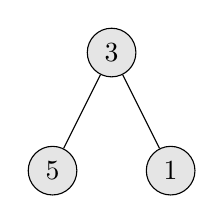
\begin{tikzpicture}
[every node/.style={draw, circle, fill=gray!20!, minimum size=5mm}]
\node{3}
child{node{5}}
child{node{1}};
\end{tikzpicture}
\end{figure}

The path sum is $(3 + 5) + (3 + 1) = 12$.
\end{flushleft}

 

\paragraph{Example 2:}

\begin{flushleft}
\textbf{Input}: \lstinline[language=C++, basicstyle=\small\ttfamily, keywordstyle=\bfseries\color{green!40!black}]|[113, 221]|

\textbf{Output}: 4

\textbf{Explanation}: 

The tree that the list represents is: 

\begin{figure}[H]
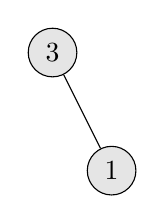
\begin{tikzpicture}
[every node/.style={draw, circle, fill=gray!20!, minimum size=5mm}]
\node{3}
child[missing]
child{node{1}};
\end{tikzpicture}
\end{figure}

The path sum is $(3 + 1) = 4$.
\end{flushleft}

\subsection{Breadth First Search}
For a full binary tree, at level $x$, there will be $2^{x-1}$ nodes.

\subsection{Breadth First Search}
For a full binary tree, at level $x$, there will be $2^{x-1}$ nodes.

\begin{enumerate}
\item Get the maximum level, say $Y$, by parsing the last element of input array $A$.
\item Iterate from level 1 to $Y$. At each level $x$
\begin{itemize}
\item Create an array, say $T$,  with size $2^{x-1}$ to save each node's accumulated sum from its parent node. 
\item If a node's position in current level is $P$, we can get its parent's index by $(P-1)/2$ since $P$ is starting with 1.
\item Add the value of its parent node to this node's own value and save to $T[P-1]$ since $P$ is starting with 1.
\item To avoid neglecting those nodes that don't have child nodes when processing next level (since we are swap $T$ to last level array), we put indices of the parent nodes with children into a hash set $S$. 
\item After complete processing whole nodes in current level, we accumulate the values of parent nodes without children into $z$ which is used to maintain the sum of those nodes without children. This is done by checking if a parent node's index is in the hash set $S$ or not.
\item Swap $T$ with another array, say $U$, which represents parent nodes.
\end{itemize}
\item Finally, we summation all the values of $U$ which contains the last level's nodes, and plus $z$.
\end{enumerate}
